\documentclass[12pt]{tufte-book}

\input header2.tex

\input defs2.tex


\begin{document}

\mainmatter

\section{This}


Lorem ipsum dolor sit amet, consectetur adipiscing elit. Sed nibh lectus, interdum sed accumsan in, pretium sit amet lectus. In malesuada sagittis hendrerit. Aliquam pretium nibh tincidunt erat iaculis vestibulum. Aenean egestas cursus justo sed convallis. Quisque nisl massa, tincidunt vel dignissim id, vulputate ut nibh. Vestibulum ante ipsum primis in faucibus orci luctus et ultrices posuere cubilia Curae; Suspendisse sit amet arcu risus. Nullam vehicula, quam nec lobortis faucibus, erat velit luctus lacus, et varius tellus tellus vitae sem. Pellentesque habitant morbi tristique senectus et netus et malesuada fames ac turpis egestas. Aenean placerat enim vitae eros pharetra eget tempor mi dignissim.

Aliquam at justo eget tellus scelerisque iaculis. Aliquam venenatis massa eu est eleifend scelerisque. Praesent ornare est ullamcorper lorem rutrum nec vulputate arcu pulvinar. Etiam lorem augue, dapibus eget cursus pellentesque, semper sed nunc. Proin lorem justo, feugiat ornare gravida non, rhoncus a nisl. Maecenas varius, urna sed congue consequat, quam nisl laoreet arcu, eget lacinia tortor felis sit amet lacus. Maecenas non purus nisl, quis euismod magna. Etiam hendrerit, ante ut imperdiet mollis, arcu ante consequat erat, vel mollis elit nulla at eros. Cras ipsum lacus, hendrerit a ullamcorper ut, molestie et sapien. Etiam vestibulum, velit a aliquam pulvinar, lectus risus placerat dolor, feugiat commodo quam lacus iaculis turpis. Integer tempor elit eu justo feugiat eget semper tortor venenatis. Fusce id augue a augue scelerisque porttitor. Sed sit amet pharetra lacus.

\section{Redundancies}

Control systems on critical applications (nuclear power plants, aircraft, etc...) have built-in redundancies.  If we build an application with, say, two redundancies that each independently fail only 1\ of the time, what is the probability that both of them will fail?  If we increase the number of redundancies to four, what is the probability that both of them will fail?  

\section{Two Girls}

\example{Say you know a family has two children, and further that at least one of them is a girl. What is the probability that they have two girls?}

An easy way to do this is to list out the possibilities:
\bi
\i Boy-Girl
\i Girl-Boy
\i Girl-Girl
\ei 
so you end up with 1 chance out of 3, or $p=0.33$.

Notice this is different than, the following

\example{Say you know a family has two children, and the first child is a girl.  What is the probability that the second child is a girl?}

This is just $p=0.5$, because the two events are independent.  Why not for the previous example?  It's because saying {\em at least one of them} counts the girls differently, and we have to take out the case of girl-girl because otherwise it is counted twice.  

\section{Cancer in Families}

Murphy, Abbey, Cancer in Families (pg 182 and 195 in Berry).  

\section{Wason Four-Card Problem}

There is an interesting problem in logic, referred to as the Wason Four-Card Problem\cite{Wason:1971fk}, involving hypothesis testing.  It is different than the hypothesis testing we've covered elsewhere because it involves the proper choice of which hypotheses to test given limited resources.  Further, it highlights an interesting bias in the typical reasoning of most people.  One version of the problem is the following.

\begin{quote}
You are given the four cards shown in Figure~\ref{fig:wagon}, and are told two rules about these cards:

\begin{marginfigure}
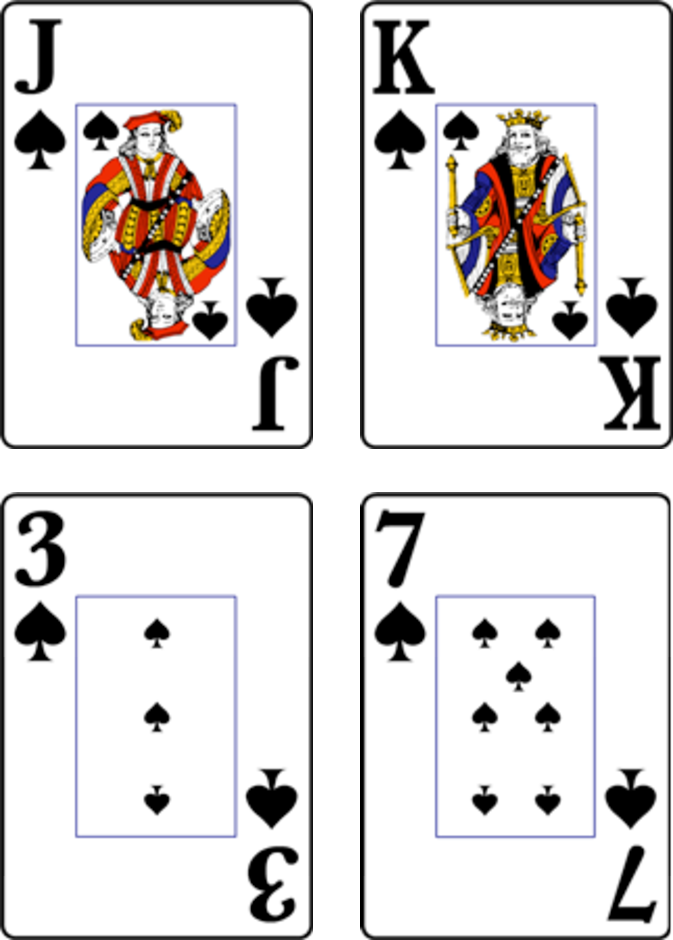
\includegraphics[width=1.2in]{wason}
\caption{Four cards for the Wason problem.}\label{fig:wagon}
\end{marginfigure}
\be
\i Each card has a {\em face card} on one side and a {\em number} on the other side.
\i If a card shows a {\em jack}, then the other side {\em must have a 3}.
\ee
Assume you can absolutely trust Rule \#1, but you want to test the truth of Rule \#2, {\em which cards would you flip over to inspect the other side?}
\end{quote}

Most people, given this task, choose $J\spades$ and $3\spades$.  Unfortunately this is a common logical fallacy called {\em Assuming the Consequent}. \marginnote{{\em Assuming the Consequent fallacy}.  This fallacy occurs when people mistake increased probability with certainty.  It takes the form  {\em if $P$ is true then $Q$ is true.  $Q$ is determined to be true, therefore $P$ is true.}  Logically this is invalid, and can be seen with a simple example:  if it is Wednesday then the banks are open.  I determine that the banks are open today, therefore today is Wednesday.  Logically this doesn't follow, but it does follow if we insert a single short phrase: if it is Wednesday the banks are open.  I determine that the banks are open today, therefore today is {\em more likely to be} Wednesday.}
The correct answer can be seen by looking at the consequences of Rule \#2, or how likely the new data (i.e. the value on the other side) is predicted from rule \#2.  Since there are four possibilities (one for each card choice I can make), we outline each one. 
\be
\i[$J\spades$:]   In this case there are two possibilities - either the other side is a $3$ or the other side is {\em not a $3$}.  The probabilities are simply:
\beqn
\Pg{J$\spades$,3 other side}{Rule \#2}&=& 1 \\
\Pg{J$\spades$,{\bf not} 3 other side}{Rule \#2}&=& 0
\eeqn
\i[$K\spades$:]   In this case there are two possibilities - either the other side is a $3$ or the other side is {\em not a $3$}.  The probabilities are simply:
\beqn
\Pg{K$\spades$,3 other side}{Rule \#2}&=&\P{K$\spades$,3 other side}  \\
\Pg{K$\spades$,{\bf not} 3 other side}{Rule \#2}&=& \P{K$\spades$,{\bf not} 3 other side}
\eeqn
where the Rule \#2 doesn't even speak about Kings, so other side probabilities are simply unaffected by it, and thus flipping this card cannot tell us anything about the rule.
\i[$3\spades$:]  In this case there are two possibilities - either the other side is a $J$ or the other side is {\em not a $J$}.  The first possibility could be a confirming example of Rule \#2, and it may be {\em more likely} to be a jack on the other side given Rule \#2 than if we didn't have Rule \#2:
\beqn
\Pg{3$\spades$,J other side}{Rule \#2}&>&\P{3$\spades$,J other side}
\eeqn
but there are other ways we could have a $3$ on one side, (3$\spades$,$K$ other side) and  (3$\spades$,$Q$ other side).  Thus, it doesn't confirm or deny Rule \#2.

What about the other possibility: {\em not a $J$} on the other side?  Here again, the best we can do is state that it is less likely for there not to be a jack on the other side with Rule \#2 then without it:
\beqn
\Pg{3$\spades$,{\bf not} J other side}{Rule \#2}&<&\P{3$\spades$,{\bf not} J other side}
\eeqn
\i[$7\spades$:]  In this case there are two possibilities - either the other side is a $J$ or the other side is {\em not a $J$}.  Notice how the probabilities here are certain and thus obtain the strength of logical conclusions:
\beqn
\Pg{7$\spades$,J other side}{Rule \#2}&=&0 \\
\Pg{7$\spades$,{\bf not} J other side}{Rule \#2}&=&1
\eeqn
\ee

So we see the correct, informative tests are $J\spades$ and $7\spades$, not $J\spades$ and $3\spades$.  

\subsection{Why is this unintuitive?}

Most people look for {\em confirming evidence} for a hypothesis.  Flipping the $J\spades$ and seeing a 3, and then flipping the $3\spades$ and seeing a jack would seem to confirm Rule \#2, even though from the above analysis we can see that it doesn't.  It would, however, make you more confident in Rule \#2, thus the {\em direction} of the inference is correct, but the {\em magnitude} of the inference is not.  Confirming evidence, although good, is not the most useful.

In science, one looks for {\em disconfirming evidence}, often referred to as {\em falsification}.  While confirming evidence might increase our confidence in a hypothesis (possibly only by a little bit), {\em disconfirming evidence} has the possibility of ruling it out entirely.  It is thus the case that hypotheses in science can never be shown to be true ($P(H)=1$) - only more likely.  However, they can be shown to be false, if they lead to predictions that are {\em not} borne out.  

\subsection{An interesting wrinkle}

An interesting variant of the same problem highlights another aspect of our psychology.  The variant is the following:
\begin{quote}
You are given the four cards shown here:
\be
\i (beer)
\i (cola)
\i (16)
\i (24)
\ee
and are told two rules about these cards:
\be
\i Each card has a {\em beverage} on one side and the drinker's {\em age}  on the other side.
\i If a person is drinking beer, then they must be over 21 years old. 
\ee
Assume you can absolutely trust Rule \#1, but you want to test the truth of Rule \#2, {\em which cards would you flip over to inspect the other side?}
\end{quote}
Here, everyone chooses correctly: [beer] and [16].  Here a possible explanation is that humans, because of evolutionary influences, can recognize {\em cheaters} and the conditions where it arises, so can evaluate these cases more readily.  It is also possible that by including a more real-world example, the logical connections are easier to parse.  Either way, there is more to probability than immediately meets the eye!

\end{document}
